% Figure 1 v8 — Wang KBS layout: 3 stacked rows (full-width per row).
% Row 1: Stage A · Inputs (3 horizontal panels)
% Row 2: Stage B · Encoder (3 horizontal panels: static / dynamic / fusion)
% Row 3: Stage C · Choice head + Loss + Trained Θ output card
%
% Compile:  pdflatex figure1_architecture_v8.tex

\documentclass[border=8pt]{standalone}

\usepackage[T1]{fontenc}
\usepackage{lmodern}
\usepackage{amsmath, amssymb}
\usepackage{tikz}
\usepackage{xcolor}
\usepackage{graphicx}

\usetikzlibrary{
  positioning, arrows.meta, shapes.geometric, calc, fit, backgrounds,
  matrix, decorations.pathmorphing,
}

\definecolor{stageABg}    {HTML}{E0EBF5}
\definecolor{stageABanner}{HTML}{3B6FB6}
\definecolor{stageBBg}    {HTML}{E6F1E5}
\definecolor{stageBBanner}{HTML}{2E7D32}
\definecolor{stageCBg}    {HTML}{FAE5DD}
\definecolor{stageCBanner}{HTML}{C44E52}
\definecolor{cFlow}       {HTML}{E07A5F}
\definecolor{cBack}       {HTML}{8B5CF6}
\definecolor{cText}       {HTML}{1F2937}
\definecolor{cMuted}      {HTML}{6B7280}
\definecolor{cBorder}     {HTML}{CBD5E1}
\definecolor{cIO}         {HTML}{0F766E}

% Tensor cell category colours
\definecolor{cPOI}      {HTML}{93C5FD}
\definecolor{cSector}   {HTML}{86EFAC}
\definecolor{cEmp}      {HTML}{FDBA74}
\definecolor{cPop}      {HTML}{FDE68A}
\definecolor{cIMD}      {HTML}{FCA5A5}
\definecolor{cTube}     {HTML}{C4B5FD}

% Mixture utility 4-term colours
\definecolor{cTermV}    {HTML}{8172B2}
\definecolor{cTermBeta} {HTML}{C44E52}
\definecolor{cTermGamma}{HTML}{F59E0B}
\definecolor{cTermDelta}{HTML}{0E7490}

% Parameter category colours
\definecolor{cParEnc}   {HTML}{475569}
\definecolor{cParBeta}  {HTML}{C44E52}
\definecolor{cParGamma} {HTML}{F59E0B}
\definecolor{cParDelta} {HTML}{0E7490}
\definecolor{cParKappa} {HTML}{8172B2}

% Agent type colours (consistent with agent_heterogeneity icon)
\definecolor{cAgentWalk}   {HTML}{10B981}
\definecolor{cAgentTransit}{HTML}{F59E0B}
\definecolor{cAgentCar}    {HTML}{3B82F6}

\newcommand{\rowwidth}{300mm}    % uniform row width

\begin{document}

\begin{tikzpicture}[
  font=\sffamily\small,
  thick,
  >={Stealth[length=4.5pt, width=4pt]},
  every node/.style={align=center, text=cText},
  %
  rowframe/.style={
    draw=none, fill=#1, rounded corners=6pt,
    inner xsep=8pt, inner ysep=10pt,
  },
  rowbanner/.style={
    fill=#1, text=white, font=\sffamily\bfseries\small,
    rounded corners=4pt, inner sep=6pt,
  },
  modA/.style={
    draw=stageABanner, fill=white, line width=0.7pt,
    rounded corners=3pt, inner sep=5pt,
  },
  modB/.style={
    draw=stageBBanner, fill=white, line width=0.7pt,
    rounded corners=3pt, inner sep=5pt,
  },
  modC/.style={
    draw=stageCBanner, fill=white, line width=0.7pt,
    rounded corners=3pt, inner sep=5pt,
  },
  arrFwd/.style={->, line width=1.6pt, draw=cFlow},
  arrInner/.style={->, line width=0.8pt, draw=cText!70},
  arrBack/.style={->, line width=1.0pt, draw=cBack, dashed},
  arrlbl/.style={font=\sffamily\scriptsize\itshape, text=cMuted, fill=white,
                 inner sep=1pt, midway},
  cellgrid/.style={draw=cMuted!50, fill=#1, line width=0.3pt, rectangle},
]

% ════════════════════════════════════════════════════════════════════════
%  ROW 1 · STAGE A · INPUTS  (7 horizontal panels with encoder/choice divider)
%  Left group  (3 panels): X^static, X^dyn, G — go through ENCODER
%  Right group (4 panels): t^(m), log d, OccMatch, π_m+π_k — skip encoder,
%                          go DIRECTLY to choice head
% ════════════════════════════════════════════════════════════════════════

\begin{scope}[local bounding box=row1]

  % ────────── LEFT GROUP: ENCODER INPUTS ──────────

  % Panel 1: Static features (text content + small matrix preview)
  \node[modA, anchor=north west] (xstatic) at (0, 0)
    {\begin{minipage}{52mm}
      \centering\textbf{\textcolor{stageABanner}{Static features}}\\
      \scriptsize $X^{\text{static}}\!\in\!\mathbb{R}^{N\!\times\!22}$\;·\;time-invariant\\[3pt]
      \raggedright\scriptsize
      \textcolor{cPOI!50!black}{$\bullet$} POI counts (office · retail · F\&B · other)\\
      \textcolor{cSector!60!black}{$\bullet$} Sectoral employment ($\times$\,8 sectors)\\
      \textcolor{cEmp!60!black}{$\bullet$} Total employment $+$ density\\
      \textcolor{cPop!60!black}{$\bullet$} Population density\\
      \textcolor{cIMD!60!black}{$\bullet$} IMD income decile\\
      \textcolor{cTube!60!black}{$\bullet$} Tube / station distance ($\times$\,5)\\[3pt]
      \centering\begin{tikzpicture}[scale=0.7, baseline=0]
        \foreach \r in {0,...,3} {
          \foreach \c in {0,1,2,3}
            \node[cellgrid=cPOI, minimum size=2mm] at (\c*2mm, -\r*2mm) {};
          \foreach \c [evaluate=\c as \cc using int(\c+4)] in {0,...,7}
            \node[cellgrid=cSector, minimum size=2mm] at (\cc*2mm, -\r*2mm) {};
          \foreach \c [evaluate=\c as \cc using int(\c+12)] in {0,1}
            \node[cellgrid=cEmp, minimum size=2mm] at (\cc*2mm, -\r*2mm) {};
          \foreach \c [evaluate=\c as \cc using int(\c+14)] in {0,1}
            \node[cellgrid=cPop, minimum size=2mm] at (\cc*2mm, -\r*2mm) {};
          \node[cellgrid=cIMD, minimum size=2mm] at (16*2mm, -\r*2mm) {};
          \foreach \c [evaluate=\c as \cc using int(\c+17)] in {0,...,4}
            \node[cellgrid=cTube, minimum size=2mm] at (\cc*2mm, -\r*2mm) {};
        }
        \node[font=\sffamily\tiny, text=cMuted] at (10*2mm, -5*2mm) {$\vdots\;N\!=\!1725$};
      \end{tikzpicture}
    \end{minipage}};

  % Panel 2: Dynamic features (text content + small cube preview)
  \node[modA, anchor=north west] (xdyn) at (62mm, 0)
    {\begin{minipage}{52mm}
      \centering\textbf{\textcolor{stageABanner}{Dynamic features}}\\
      \scriptsize $X^{\text{dyn}}\!\in\!\mathbb{R}^{T\!\times\!N\!\times\!5}$\;·\;hourly\\[3pt]
      \raggedright\scriptsize
      \textcolor{stageABanner}{$\bullet$} Hourly congestion (z-scored)\\
      \textcolor{stageABanner}{$\bullet$} Hourly destination inflow (z)\\
      \textcolor{stageABanner}{$\bullet$} Queue residual (placeholder)\\
      \textcolor{stageABanner}{$\bullet$} Cyclic time: $\sin h$, $\cos h$\\[3pt]
      \centering\begin{tikzpicture}[baseline=0]
        \foreach \r in {0,...,3} {
          \foreach \c in {0,...,4} {
            \node[cellgrid=stageABanner, minimum size=2.0mm,
                   opacity={0.30+0.15*\r}]
                  at (\c*2.0mm, -\r*2.0mm) {};
          }
        }
        \draw[fill=stageABanner!30, opacity=0.6, line width=0.3pt]
          (0, 0.8mm) -- (5*2.0mm, 0.8mm) -- (5*2.0mm + 6mm, 4mm) -- (6mm, 4mm) -- cycle;
        \draw[fill=stageABanner!20, opacity=0.6, line width=0.3pt]
          (5*2.0mm, 0.8mm) -- (5*2.0mm + 6mm, 4mm)
            -- (5*2.0mm + 6mm, 4mm - 4*2.0mm) -- (5*2.0mm, -3*2.0mm) -- cycle;
        \node[font=\sffamily\tiny, text=cMuted] at (-3mm, -3mm) {$N$};
        \node[font=\sffamily\tiny, text=cMuted] at (5mm, 5mm) {$T\!=\!24$};
        \node[font=\sffamily\tiny, text=cMuted] at (5*2.0mm + 8mm, -2mm) {$F\!=\!5$};
      \end{tikzpicture}
    \end{minipage}};

  % Panel 3: G (graph)
  \node[modA, anchor=north west] (xgraph) at (124mm, 0)
    {\begin{minipage}{40mm}
      \centering\textbf{\textcolor{stageABanner}{$\mathcal{G}\!=\!(V,E)$}}\;\\\tiny\textcolor{cMuted}{edge\_index, derived}\\[3pt]
      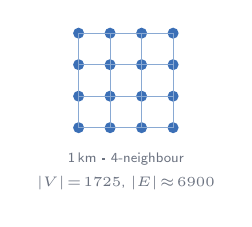
\begin{tikzpicture}[baseline=0]
        \foreach \x/\y/\name in
          {0/0/n00, 1/0/n10, 2/0/n20, 3/0/n30,
           0/1/n01, 1/1/n11, 2/1/n21, 3/1/n31,
           0/2/n02, 1/2/n12, 2/2/n22, 3/2/n32,
           0/3/n03, 1/3/n13, 2/3/n23, 3/3/n33}{
          \node[circle, fill=stageABanner, minimum size=1.4mm, inner sep=0pt]
                (\name) at (\x*4mm, -\y*4mm) {};
        }
        \foreach \y in {0,1,2,3}{
          \foreach \x in {0,1,2}{
            \pgfmathtruncatemacro{\xn}{\x+1}
            \draw[stageABanner!60, line width=0.3pt] (\x*4mm, -\y*4mm) -- (\xn*4mm, -\y*4mm);
          }
        }
        \foreach \x in {0,1,2,3}{
          \foreach \y in {0,1,2}{
            \pgfmathtruncatemacro{\yn}{\y+1}
            \draw[stageABanner!60, line width=0.3pt] (\x*4mm, -\y*4mm) -- (\x*4mm, -\yn*4mm);
          }
        }
        \node[font=\sffamily\tiny, text=cMuted] at (6mm, -16mm) {1\,km · 4-neighbour};
        \node[font=\sffamily\tiny, text=cMuted] at (6mm, -19mm) {$|V|\!=\!1725$, $|E|\!\approx\!6900$};
      \end{tikzpicture}
    \end{minipage}};

\end{scope}

% Stage A frame (left 3 panels — encoder inputs only)
\begin{pgfonlayer}{background}
  \node[rowframe=stageABg, fit=(row1)] (frameRow1) {};
\end{pgfonlayer}
\node[rowbanner=stageABanner, anchor=north west]
  at ($(frameRow1.north west)+(8pt, 0pt)$)
  {\textsc{Stage A · Encoder inputs}\;\,\textmd{\itshape — fed into encoder (Stage B) below}};

% ════════════════════════════════════════════════════════════════════════
%  RIGHT COLUMN · CHOICE-HEAD INPUTS (vertical stack, parallel to Stage A+B)
%  Bypass the encoder; feed directly into Stage C choice head.
% ════════════════════════════════════════════════════════════════════════

\begin{scope}[local bounding box=rightcol, shift={(186mm, 0)}]

  % R1: Travel time per mode
  \node[modA, anchor=north west, draw=stageBBanner] (tij) at (0, 0)
    {\begin{minipage}{96mm}
      \centering\textbf{\textcolor{stageBBanner}{Travel time per mode}}\;\scriptsize $t_{ij}^{(m)}\!\in\!\mathbb{R}^{N\!\times\!N\!\times\!3}$\\
      \tiny\textcolor{cMuted}{free-flow car / transit / walk · OD-pair travel time}\\[3pt]
      \begin{tikzpicture}[baseline=0]
        \foreach \mname/\yoff/\col in {car/0/cAgentCar, transit/-7mm/cAgentTransit, walk/-14mm/cAgentWalk}{
          \node[font=\sffamily\tiny, text=\col, anchor=east] at (-1mm, \yoff) {\mname};
          \foreach \c in {0,...,29}{
            \pgfmathsetmacro{\val}{0.15 + 0.025*\c}
            \node[cellgrid=cTermBeta, minimum size=1.5mm, opacity=\val]
                  at (\c*1.5mm, \yoff) {};
          }
        }
        \node[font=\sffamily\tiny, text=cMuted] at (24mm, -19mm)
              {feeds $\beta_{t,m}\!\cdot\! t_{ij}^{(m)}$ in choice head};
      \end{tikzpicture}
    \end{minipage}};

  % R2: OccMatch — pushed lower so right column spans Stage A + Stage B vertically
  \node[modA, anchor=north west, draw=stageBBanner] (occm) at (0, -65mm)
    {\begin{minipage}{96mm}
      \centering\textbf{\textcolor{stageBBanner}{Occupational matching}}\;\scriptsize OccMatch$_{ij}\!\in\!\mathbb{R}^{N\!\times\!N}$\\
      \tiny\textcolor{cMuted}{cosine similarity, origin SOC9 $\times$ destination sector}\\[3pt]
      \begin{tikzpicture}[baseline=0]
        \foreach \r in {0,...,5}{
          \foreach \c in {0,...,17}{
            \pgfmathsetmacro{\val}{0.1 + 0.5*rnd}
            \node[cellgrid=cTermDelta, minimum size=1.5mm, opacity=\val]
                  at (\c*1.5mm, -\r*1.5mm) {};
          }
        }
        \node[font=\sffamily\tiny, text=cMuted] at (14mm, -12mm)
              {feeds $\delta_k\!\cdot\!$OccM in choice head};
      \end{tikzpicture}
    \end{minipage}};

  % R3: Heterogeneity priors π_m + π_k — bottom of right column, aligned with Stage B bottom
  \node[modA, anchor=north west, draw=stageBBanner] (pies) at (0, -130mm)
    {\begin{minipage}{96mm}
      \centering\textbf{\textcolor{stageBBanner}{Heterogeneity priors}}\;\scriptsize $\pi_m(i,j),\,\pi_k(i)$\\
      \tiny\textcolor{cMuted}{mode share + income tier per origin}\\[3pt]
      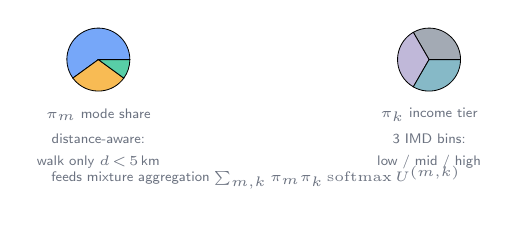
\begin{tikzpicture}[baseline=0]
        \begin{scope}[shift={(8mm, -3mm)}]
          \draw[fill=cAgentCar!70, line width=0.3pt] (0,0) -- (0:4mm) arc (0:216:4mm) -- cycle;
          \draw[fill=cAgentTransit!70, line width=0.3pt] (0,0) -- (216:4mm) arc (216:324:4mm) -- cycle;
          \draw[fill=cAgentWalk!70, line width=0.3pt] (0,0) -- (324:4mm) arc (324:360:4mm) -- cycle;
          \node[font=\sffamily\tiny, text=cMuted] at (0, -7mm) {$\pi_m$ mode share};
          \node[font=\sffamily\tiny, text=cMuted] at (0, -10mm) {distance-aware:};
          \node[font=\sffamily\tiny, text=cMuted] at (0, -13mm) {walk only $d\!<\!5$\,km};
        \end{scope}
        \begin{scope}[shift={(50mm, -3mm)}]
          \draw[fill=cParEnc!50, line width=0.3pt] (0,0) -- (0:4mm) arc (0:120:4mm) -- cycle;
          \draw[fill=cParKappa!50, line width=0.3pt] (0,0) -- (120:4mm) arc (120:240:4mm) -- cycle;
          \draw[fill=cParDelta!50, line width=0.3pt] (0,0) -- (240:4mm) arc (240:360:4mm) -- cycle;
          \node[font=\sffamily\tiny, text=cMuted] at (0, -7mm) {$\pi_k$ income tier};
          \node[font=\sffamily\tiny, text=cMuted] at (0, -10mm) {3 IMD bins:};
          \node[font=\sffamily\tiny, text=cMuted] at (0, -13mm) {low / mid / high};
        \end{scope}
        \node[font=\sffamily\tiny, text=cMuted] at (28mm, -18mm)
              {feeds mixture aggregation $\sum_{m,k}\pi_m\pi_k\,\mathrm{softmax}\,U^{(m,k)}$};
      \end{tikzpicture}
    \end{minipage}};

\end{scope}

\begin{pgfonlayer}{background}
  \node[rowframe=stageBBg, fit=(rightcol)] (frameRightCol) {};
\end{pgfonlayer}
\node[rowbanner=stageBBanner, anchor=north west]
  at ($(frameRightCol.north west)+(8pt, 0pt)$)
  {\textsc{Choice-head inputs}\;\,\textmd{\itshape — bypass the encoder, feed directly to Stage C}};

% ════════════════════════════════════════════════════════════════════════
%  ROW 2 · STAGE B · ENCODER  (static / dynamic / fusion horizontal)
% ════════════════════════════════════════════════════════════════════════

\begin{scope}[local bounding box=row2, shift={(0, -80mm)}]

  % ── ① Static branch ──
  \node[modB, anchor=north west] (sage) at (0, 0)
    {\begin{minipage}{52mm}
      \centering\textbf{\textcolor{stageBBanner}{\textcircled{\scriptsize 1} Static branch · GraphSAGE $\times 2$}}\\[1pt]
      \scriptsize\textcolor{cIO}{IN: $X^{\text{static}}, \mathcal{G}$}\;\;\textcolor{cIO}{OUT: $h_s\!\in\!\mathbb{R}^{N\!\times\!32}$}\\[3pt]
      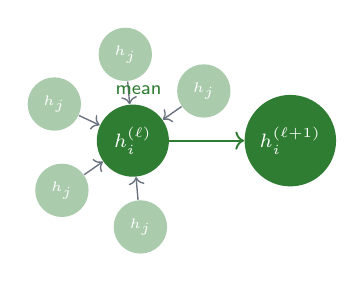
\begin{tikzpicture}[baseline=0]
        \node[circle, fill=stageBBanner, minimum size=6mm, font=\sffamily\scriptsize, text=white]
          (hi) at (0, 0) {$h_i^{(\ell)}$};
        \foreach \angle/\name in {35/n1, 95/n2, 155/n3, 215/n4, 275/n5}{
          \node[circle, fill=stageBBanner!40, minimum size=4mm,
                 font=\sffamily\tiny, text=white]
                (\name) at ({\angle}:11mm) {$h_j$};
          \draw[->, line width=0.5pt, draw=cMuted] (\name) -- (hi);
        }
        \node[font=\sffamily\scriptsize, text=stageBBanner, anchor=south]
           at (hi.north) {\;\;mean};
        \node[circle, fill=stageBBanner, minimum size=6mm, font=\sffamily\scriptsize, text=white]
          (hi1) at (20mm, 0) {$h_i^{(\ell{+}1)}$};
        \draw[->, line width=0.7pt, draw=stageBBanner] (hi.east) -- (hi1.west);
      \end{tikzpicture}\\[2pt]
      \scriptsize $h_i^{(\ell+1)}=\sigma\big(W^{(\ell)}\!\cdot\!\mathrm{mean}_{j\in\mathcal{N}(i)} h_j^{(\ell)}\big)$\\
      \tiny\textcolor{cMuted}{layer 1: $W^{(1)}{:}\,22{\to}32$;\;\;layer 2: $W^{(2)}{:}\,32{\to}32$}
    \end{minipage}};

  % ── ② Dynamic branch (compressed to fit Stage A width) ──
  \node[modB, anchor=north west] (dyn) at (60mm, 0)
    {\begin{minipage}{106mm}
      \centering\textbf{\textcolor{stageBBanner}{\textcircled{\scriptsize 2} Dynamic branch · per-hour SAGE $\to$ GRU $\to$ multi-scale TCN $\to$ fuse}}\\[1pt]
      \scriptsize\textcolor{cIO}{IN: $X^{\text{dyn}}, \mathcal{G}$}\;\;\textcolor{cIO}{OUT: $h_d\!\in\!\mathbb{R}^{T\!\times\!N\!\times\!32}$}\\[3pt]
      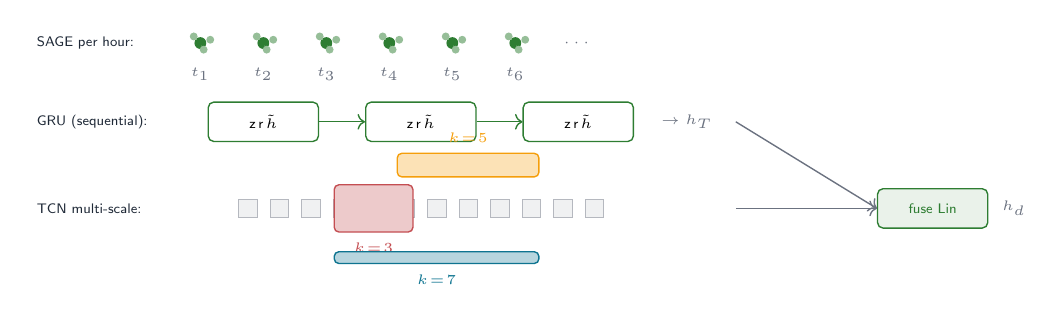
\begin{tikzpicture}[baseline=0]
        % per-hour SAGE
        \node[font=\sffamily\tiny, text=cText, anchor=west] at (0, 18mm) {SAGE per hour:};
        \foreach \t/\xoff in {1/22, 2/30, 3/38, 4/46, 5/54, 6/62}{
          \begin{scope}[shift={(\xoff mm, 18mm)}, scale=0.42]
            \node[circle, fill=stageBBanner, minimum size=1.5mm, inner sep=0pt] (a\t) at (0,0) {};
            \node[circle, fill=stageBBanner!50, minimum size=1.0mm, inner sep=0pt] (b\t) at (3mm, 1mm) {};
            \node[circle, fill=stageBBanner!50, minimum size=1.0mm, inner sep=0pt] (c\t) at (-2mm, 2mm) {};
            \node[circle, fill=stageBBanner!50, minimum size=1.0mm, inner sep=0pt] (d\t) at (1mm, -2mm) {};
            \draw[stageBBanner!50, line width=0.2pt] (a\t)--(b\t) (a\t)--(c\t) (a\t)--(d\t);
          \end{scope}
          \node[font=\sffamily\tiny, text=cMuted] at (\xoff mm, 14mm) {$t_\t$};
        }
        \node[font=\sffamily\tiny, text=cMuted] at (70mm, 18mm) {$\cdots$};
        % GRU row
        \node[font=\sffamily\tiny, text=cText, anchor=west] at (0, 8mm) {GRU (sequential):};
        \foreach \t/\xoff in {1/30, 2/50, 3/70}{
          \node[draw=stageBBanner, rounded corners=2pt, fill=white, line width=0.5pt,
                 minimum width=14mm, minimum height=5mm,
                 font=\sffamily\tiny] (gru\t) at (\xoff mm, 8mm) {z\,r\,$\tilde h$};
        }
        \draw[->, line width=0.5pt, draw=stageBBanner] (gru1.east) -- (gru2.west);
        \draw[->, line width=0.5pt, draw=stageBBanner] (gru2.east) -- (gru3.west);
        \node[font=\sffamily\tiny, text=cMuted] at (84mm, 8mm) {$\!\to h_T$};
        % TCN row
        \node[font=\sffamily\tiny, text=cText, anchor=west] at (0, -3mm) {TCN multi-scale:};
        \foreach \i in {0,...,11}{
          \node[draw=cMuted!50, fill=cMuted!10, minimum size=2mm, line width=0.2pt]
                at (28mm + \i*4mm, -3mm) {};
        }
        \draw[draw=cTermBeta, fill=cTermBeta!30, line width=0.5pt, rounded corners=0.6mm]
              (28mm + 3*4mm - 1mm, -6mm) rectangle (28mm + 5*4mm + 1mm, 0mm);
        \node[font=\sffamily\tiny, text=cTermBeta] at (28mm + 4*4mm, -8mm) {$k\!=\!3$};
        \draw[draw=cTermGamma, fill=cTermGamma!30, line width=0.5pt, rounded corners=0.6mm]
              (28mm + 5*4mm - 1mm, 1mm) rectangle (28mm + 9*4mm + 1mm, 4mm);
        \node[font=\sffamily\tiny, text=cTermGamma] at (28mm + 7*4mm, 6mm) {$k\!=\!5$};
        \draw[draw=cTermDelta, fill=cTermDelta!30, line width=0.5pt, rounded corners=0.6mm]
              (28mm + 3*4mm - 1mm, -10mm) rectangle (28mm + 9*4mm + 1mm, -8.5mm);
        \node[font=\sffamily\tiny, text=cTermDelta] at (28mm + 6*4mm, -12mm) {$k\!=\!7$};
        % fuse Lin
        \node[draw=stageBBanner, rounded corners=2pt, fill=stageBBanner!10,
               line width=0.5pt, minimum width=14mm, minimum height=5mm,
               font=\sffamily\tiny, text=stageBBanner]
              (fuse) at (115mm, -3mm) {fuse Lin};
        \draw[->, line width=0.5pt, draw=cMuted] (90mm, 8mm) -- (fuse.west);
        \draw[->, line width=0.5pt, draw=cMuted] (90mm, -3mm) -- (fuse.west);
        \node[font=\sffamily\tiny, text=cMuted, anchor=west] at (fuse.east) {\;$h_d$};
      \end{tikzpicture}
    \end{minipage}};

  % ── ③ Gated fusion (BELOW the two branches — sub-row 2, full Stage A width) ──
  \node[modB, anchor=north west] (gfuse) at (8mm, -68mm)
    {\begin{minipage}{156mm}
      \centering\textbf{\textcolor{stageBBanner}{\textcircled{\scriptsize 3} Gated fusion $\to V_{j,t}$}}\;\;\scriptsize\textcolor{cIO}{IN: $h_s, h_d$}\;\;\textcolor{cIO}{OUT: $V_{j,t}\!\in\!\mathbb{R}^{T\!\times\!N}$}\\[3pt]
      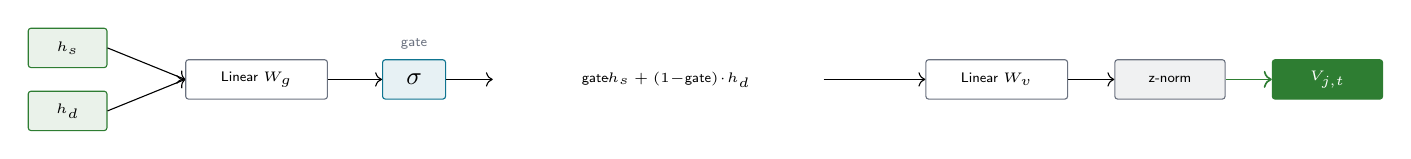
\begin{tikzpicture}[baseline=0]
        \node[draw=stageBBanner, fill=stageBBanner!10, rounded corners=1pt,
               minimum width=10mm, minimum height=5mm, font=\sffamily\tiny] (hs) at (0, 4mm) {$h_s$};
        \node[draw=stageBBanner, fill=stageBBanner!10, rounded corners=1pt,
               minimum width=10mm, minimum height=5mm, font=\sffamily\tiny] (hd) at (0, -4mm) {$h_d$};
        \node[draw=cMuted, fill=white, rounded corners=1pt,
               minimum width=18mm, minimum height=5mm, font=\sffamily\tiny] (lin) at (24mm, 0) {Linear $W_g$};
        \draw[->, line width=0.4pt] (hs.east) -- (lin.west);
        \draw[->, line width=0.4pt] (hd.east) -- (lin.west);
        \node[draw=cTermDelta, fill=cTermDelta!10, rounded corners=1pt,
               minimum width=8mm, minimum height=5mm, font=\sffamily\small] (sig) at (44mm, 0) {$\sigma$};
        \draw[->, line width=0.4pt] (lin.east) -- (sig.west);
        \node[font=\sffamily\tiny, text=cMuted, anchor=south] at (sig.north) {gate};
        \node[font=\sffamily\tiny] at (76mm, 0) {gate$\!\cdot\!h_s+(1{-}$gate$)\!\cdot\!h_d$};
        \draw[->, line width=0.4pt] (sig.east) -- (54mm, 0);
        \node[draw=cMuted, fill=white, rounded corners=1pt,
               minimum width=18mm, minimum height=5mm, font=\sffamily\tiny] (vh) at (118mm, 0) {Linear $W_v$};
        \draw[->, line width=0.4pt] (96mm, 0) -- (vh.west);
        \node[draw=cMuted, fill=cMuted!10, rounded corners=1pt,
               minimum width=14mm, minimum height=5mm, font=\sffamily\tiny] (zn) at (140mm, 0) {z-norm};
        \draw[->, line width=0.4pt] (vh.east) -- (zn.west);
        \node[draw=stageBBanner, fill=stageBBanner, rounded corners=1pt,
               minimum width=14mm, minimum height=5mm,
               font=\sffamily\tiny, text=white] (vjt) at (160mm, 0) {$V_{j,t}$};
        \draw[->, line width=0.6pt, draw=stageBBanner] (zn.east) -- (vjt.west);
      \end{tikzpicture}
    \end{minipage}};

  % arrows from Static / Dynamic branches DOWN into Gated fusion
  \draw[arrInner] (sage.south) -- node[arrlbl, right]{$h_s$} ($(gfuse.north)+(-50mm, 0)$);
  \draw[arrInner] (dyn.south)  -- node[arrlbl, right]{$h_d$} ($(gfuse.north)+(50mm, 0)$);

\end{scope}

\begin{pgfonlayer}{background}
  \node[rowframe=stageBBg, fit=(row2)] (frameRow2) {};
\end{pgfonlayer}
\node[rowbanner=stageBBanner, anchor=north west]
  at ($(frameRow2.north west)+(8pt, 0pt)$)
  {\textsc{Stage B · Encoder}\;\,\textmd{\itshape — dual-branch ST-GNN $+$ gated fusion · 33{,}026 weights}};

% ════════════════════════════════════════════════════════════════════════
%  ROW 3 · STAGE C · CHOICE HEAD + LOSS + TRAINED Θ
% ════════════════════════════════════════════════════════════════════════

\begin{scope}[local bounding box=row3, shift={(0, -180mm)}]

  % ── ④ Compute 9 utilities U^(m,k) (Stage C extends to A+rightcol total width 282mm) ──
  \node[modC, anchor=north west] (utility) at (0, 0)
    {\begin{minipage}{96mm}
      \centering\textbf{\textcolor{stageCBanner}{\textcircled{\scriptsize 4} Compute 9 utilities $U^{(m,k)}$}}\\[1pt]
      \scriptsize 1 utility per mode $\times$ tier combination\\[3pt]
      \scriptsize $U^{(m,k)}_{ij,t} =\;$\textcolor{cTermV}{$\alpha V_{j,t}$}$+$\textcolor{cTermBeta}{$\beta_{t,m}\kappa_k t_{ij}^{(m)}$}\\
      \;\;\;$+$\textcolor{cTermGamma}{$\gamma\log d_{ij}$}$+$\textcolor{cTermDelta}{$\delta_k\mathrm{OccM}_{ij}$}\\[5pt]
      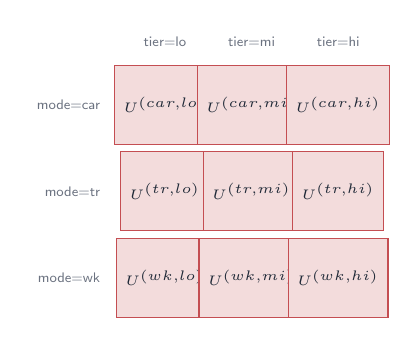
\begin{tikzpicture}[baseline=0]
        % 3x3 grid of U^(m,k) cells
        \foreach \r/\m in {0/car, 1/tr, 2/wk}{
          \foreach \c/\k in {0/lo, 1/mi, 2/hi}{
            \node[draw=cTermBeta, fill=cTermBeta!20, line width=0.4pt,
                   minimum size=10mm, font=\sffamily\tiny, text=cText]
                  (u\m\k) at (\c*11mm, -\r*11mm) {$U^{(\m,\k)}$};
          }
        }
        \foreach \c/\k in {0/lo, 1/mi, 2/hi}
          \node[font=\sffamily\tiny, text=cMuted] at (\c*11mm, 8mm) {tier=\k};
        \foreach \r/\m in {0/car, 1/tr, 2/wk}
          \node[font=\sffamily\tiny, text=cMuted, anchor=east] at (-7mm, -\r*11mm) {mode=\m};
      \end{tikzpicture}
    \end{minipage}};

  % ── ⑤ Apply softmax to each → 9 distributions ──
  \node[modC, anchor=north west] (softmax) at (102mm, 0)
    {\begin{minipage}{86mm}
      \centering\textbf{\textcolor{stageCBanner}{\textcircled{\scriptsize 5} Softmax over destinations $j$}}\\[1pt]
      \scriptsize 9 probability distributions: $\mathrm{sm}_j(U^{(m,k)})$\\[3pt]
      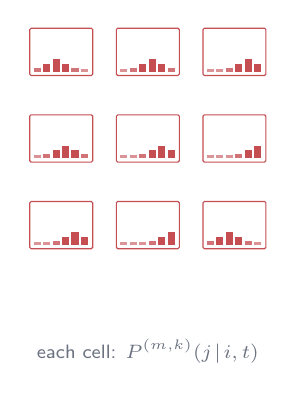
\begin{tikzpicture}[baseline=0]
        \foreach \r in {0,1,2}{
          \foreach \c in {0,1,2}{
            \begin{scope}[shift={(\c*11mm, -\r*11mm)}]
              \draw[draw=cTermBeta, fill=white, line width=0.4pt,
                     rounded corners=0.5pt]
                    (-4mm, -3mm) rectangle (4mm, 3mm);
              \pgfmathtruncatemacro{\peak}{2 + Mod(\r+\c, 4)}
              \foreach \b in {0,1,2,3,4,5}{
                \pgfmathsetmacro{\dist}{(\b-\peak)*(\b-\peak)}
                \pgfmathsetmacro{\hh}{0.6 + 2.0*exp(-0.6*\dist)}
                \fill[cTermBeta, opacity=\hh, opacity={min(\hh,1)}]
                  (-3.5mm + \b*1.2mm, -2.5mm) rectangle
                  (-3.5mm + \b*1.2mm + 0.9mm, -2.5mm + \hh*0.6mm);
              }
            \end{scope}
          }
        }
        \node[font=\sffamily\scriptsize, text=cMuted] at (11mm, -38mm) {each cell: $P^{(m,k)}(j\!\mid\!i,t)$};
      \end{tikzpicture}
    \end{minipage}};

  % ── ⑥ Mixture aggregation → P(j|i,t) ──
  \node[modC, anchor=north west] (mixture) at (194mm, 0)
    {\begin{minipage}{86mm}
      \centering\textbf{\textcolor{stageCBanner}{\textcircled{\scriptsize 6} Mixture aggregation}}\\[1pt]
      \scriptsize weighted by $\pi_m(i,j)\!\cdot\!\pi_k(i)$\\[3pt]
      \scriptsize $P(j|i,t) = \!\!\sum_{m,k}\!\pi_m(i,j)\,\pi_k(i)$\\
      \;\;$\cdot\,\mathrm{softmax}_j\,U^{(m,k)}_{ij,t}$\\[5pt]
      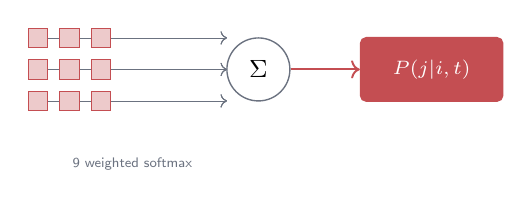
\begin{tikzpicture}[baseline=0]
        \foreach \i in {0,1,2,3,4,5,6,7,8}{
          \pgfmathtruncatemacro{\row}{int(\i/3)}
          \pgfmathtruncatemacro{\col}{Mod(\i, 3)}
          \node[draw=cTermBeta, fill=cTermBeta!30, minimum size=2.5mm, line width=0.3pt]
                (s\i) at (\col*4mm, -\row*4mm) {};
          \draw[->, line width=0.3pt, draw=cMuted] (s\i.east) -- (24mm, -\row*4mm);
        }
        \node[draw=cMuted, fill=white, circle, line width=0.5pt,
               minimum size=8mm, font=\sffamily\small]
              (sigma) at (28mm, -4mm) {$\Sigma$};
        \node[draw=cTermBeta, fill=cTermBeta, rounded corners=2pt,
               line width=0.7pt, minimum width=18mm, minimum height=8mm,
               font=\sffamily\scriptsize, text=white]
              (P) at (50mm, -4mm) {$P(j|i,t)$};
        \draw[->, line width=0.7pt, draw=cTermBeta] (sigma.east) -- (P.west);
        \node[font=\sffamily\tiny, text=cMuted] at (12mm, -16mm) {9 weighted softmax};
      \end{tikzpicture}
    \end{minipage}};

  % ── ⑦ Cross-entropy loss + backprop (compact, less prominent than ④⑤⑥) ──
  \node[modC, anchor=north west, fill=stageCBanner!8] (loss) at (60mm, -56mm)
    {\begin{minipage}{160mm}
      \centering\textbf{\textcolor{stageCBanner}{\textcircled{\scriptsize 7} Cross-entropy loss + joint backprop}}\\[1pt]
      \scriptsize $\mathcal{L} = -\!\!\sum F_{ij,t}\,\log P(j|i,t)$\;\;|\;\;
      Adam: enc lr 1e-3, head lr 1e-2\;\;|\;\;$\nabla_\Theta\mathcal{L}$ updates $\Theta_{\text{enc}} \cup (\beta,\gamma,\delta,\kappa)$\\[3pt]
      \begin{minipage}[c]{72mm}\centering
        \includegraphics[width=68mm]{../figures/arch/train_curve_v2.png}\\
        \tiny\textit{val CPC = 0.488 · London 2019 · 200 ep}
      \end{minipage}\hfill
      \begin{minipage}[c]{82mm}\raggedright\tiny
        $\bullet$ MLE on aggregate hourly OD\\
        $\bullet$ $\Theta_{\text{enc}}$ learns flexible $V_{j,t}$ from data\\
        $\bullet$ $(\beta,\gamma,\delta,\kappa)$ identified \emph{conditional on V}\\
        $\bullet$ All 33{,}103 params updated together
      \end{minipage}
    \end{minipage}};

  % inner arrows in row 3
  \draw[arrInner] (utility.east) -- node[arrlbl, above]{$U^{(m,k)}$} (softmax.west);
  \draw[arrInner] (softmax.east) -- node[arrlbl, above]{$P^{(m,k)}$} (mixture.west);
  \draw[arrInner] (mixture.south) |- node[arrlbl, near end, above]{$P(j|i,t)$} ($(loss.north)+(0,0)$);

  % backprop arrow (red dashed) — simple horizontal path
  \draw[arrBack] (loss.north west) -- ++(-12mm, 0) |-
          node[arrlbl, near end, font=\sffamily\scriptsize\itshape, fill=white, text=cBack]
              {$\nabla_\Theta\mathcal{L}$}
          (utility.west);

\end{scope}

\begin{pgfonlayer}{background}
  \node[rowframe=stageCBg, fit=(row3)] (frameRow3) {};
\end{pgfonlayer}
\node[rowbanner=stageCBanner, anchor=north west]
  at ($(frameRow3.north west)+(8pt, 0pt)$)
  {\textsc{Stage C · Choice head + Loss}\;\,\textmd{\itshape — supervised learning · 77 interpretable parameters}};

% ════════════════════════════════════════════════════════════════════════
%  ROW 4 · TRAINED Θ — output card with 5 sub-cards (full width)
% ════════════════════════════════════════════════════════════════════════

\begin{scope}[local bounding box=row4, shift={(0, -320mm)}]

  % Trained Θ cards: BIG English meaning first; math symbols + counts secondary.
  % NO row banner — the cards themselves carry the message.

  \node[draw=cParEnc, fill=cParEnc!10, rounded corners=4pt, line width=0.9pt,
         font=\sffamily\footnotesize, text=cParEnc, anchor=north west] (penc) at (0mm, 0)
     {\begin{minipage}{48mm}
      \centering\textbf{\large Encoder weights}\\
      \scriptsize\textit{deep ML representation}\\[5pt]
      \raggedright\tiny\textbullet\;encoder maps inputs $\to V_{j,t}$\\
      \textbullet\;used in every agent's encode pass\\
      \textbullet\;not directly interpretable\\[4pt]
      \centering\scriptsize $\Theta_{\text{enc}}$ · 33{,}026 weights
    \end{minipage}};

  \node[draw=cParBeta, fill=cParBeta!10, rounded corners=4pt, line width=0.9pt,
         font=\sffamily\footnotesize, text=cParBeta, anchor=north west] (pbeta) at (54mm, 0)
     {\begin{minipage}{54mm}
      \centering\textbf{\large Time sensitivity}\\
      \scriptsize\textit{per mode $\times$ per hour}\\[5pt]
      \raggedright\tiny\textbullet\;how strongly travel time deters choice\\
      \textbullet\;agent uses sensitivity for their own mode\\[3pt]
      \centering\tiny car ${-}.187$\;\;transit ${-}.105$\;\;walk ${-}.049$\\[4pt]
      \scriptsize $\beta_{t,m}$ · 72 trained values
    \end{minipage}};

  \node[draw=cParGamma, fill=cParGamma!10, rounded corners=4pt, line width=0.9pt,
         font=\sffamily\footnotesize, text=cParGamma, anchor=north west] (pgamma) at (114mm, 0)
     {\begin{minipage}{42mm}
      \centering\textbf{\large Distance decay}\\
      \scriptsize\textit{universal log-distance}\\[5pt]
      \raggedright\tiny\textbullet\;penalises long-distance OD pairs\\
      \textbullet\;shared across ALL agents\\[5pt]
      \centering\scriptsize recovered: $-0.328$\\[3pt]
      \scriptsize $\gamma$ · 1 trained scalar
    \end{minipage}};

  \node[draw=cParDelta, fill=cParDelta!10, rounded corners=4pt, line width=0.9pt,
         font=\sffamily\footnotesize, text=cParDelta, anchor=north west] (pdelta) at (160mm, 0)
     {\begin{minipage}{54mm}
      \centering\textbf{\large Occupational matching}\\
      \scriptsize\textit{by income tier}\\[5pt]
      \raggedright\tiny\textbullet\;rewards origin-occ.\,$\to$ dest-sector match\\
      \textbullet\;agent uses coefficient for their tier\\[3pt]
      \centering\tiny low $0$\;\;mid $+.20$\;\;high $+.20$\\[4pt]
      \scriptsize $\delta_k$ · 2 trained values
    \end{minipage}};

  \node[draw=cParKappa, fill=cParKappa!10, rounded corners=4pt, line width=0.9pt,
         font=\sffamily\footnotesize, text=cParKappa, anchor=north west] (pkappa) at (220mm, 0)
     {\begin{minipage}{54mm}
      \centering\textbf{\large Income tier scaling}\\
      \scriptsize\textit{multiplier on time sensitivity}\\[5pt]
      \raggedright\tiny\textbullet\;higher tiers value time more (larger $|\beta|$)\\
      \textbullet\;agent uses scaling for their tier\\[3pt]
      \centering\tiny low $1.00$\;\;mid $1.97$\;\;high $1.97$\\[4pt]
      \scriptsize $\kappa_k$ · 2 trained values
    \end{minipage}};

\end{scope}

\begin{pgfonlayer}{background}
  \node[rowframe=cParEnc!4, fit=(row4)] (frameRow4) {};
\end{pgfonlayer}

% ════════════════════════════════════════════════════════════════════════
%  MAIN VERTICAL FLOW ARROWS BETWEEN ROWS
% ════════════════════════════════════════════════════════════════════════

\draw[arrFwd] ($(frameRow1.south)+(0, 0)$) --
              node[arrlbl, fill=white, font=\sffamily\small\bfseries]{tensors}
              ($(frameRow2.north)+(0, 0)$);
\draw[arrFwd] ($(frameRow2.south)+(0, 0)$) --
              node[arrlbl, fill=white, font=\sffamily\small\bfseries]{$V_{j,t}$}
              ($(frameRow3.north)+(0, 0)$);
\draw[arrFwd] ($(frameRow3.south)+(0, 0)$) --
              node[arrlbl, fill=white, font=\sffamily\small\bfseries]{trained $\Theta$}
              ($(frameRow4.north)+(0, 0)$);

% ════════════════════════════════════════════════════════════════════════
%  Title and footer
% ════════════════════════════════════════════════════════════════════════

\node[font=\sffamily\bfseries\Large, anchor=south west, text=cText]
  at ($(frameRow1.north west)+(0, 8mm)$)
  {Figure 1 — ML Training Pipeline};
\node[font=\sffamily\itshape\large, anchor=south west, text=cMuted]
  at ($(frameRow1.north west)+(0, 4mm)$)
  {supervised inverse learning of choice parameters from aggregate hourly OD};

\node[font=\sffamily\scriptsize\itshape, text=cMuted, anchor=north west,
       text width=300mm]
  at ($(frameRow4.south west)+(0, -6pt)$)
  {Trained $\Theta$ has \textbf{5 functional categories}:
   $\Theta_{\text{enc}}$ (deep ML, used by anyone going through encoder);
   $\beta_{t,m}$ (time sensitivity, fetched per agent's mode);
   $\gamma$ (distance, shared);
   $\delta_k$ (occ.\ match, fetched per tier);
   $\kappa_k$ (tier scaling on $\beta$, fetched per tier).
   These five types bridge to Figure~2 (ABM forward simulation).};

\end{tikzpicture}

\end{document}
